\documentclass{article}
\usepackage{amsmath}
\usepackage{amssymb}
\usepackage[slovak]{babel}
\usepackage[utf8]{inputenc}
\usepackage{amsfonts}
\usepackage{graphicx}
\usepackage{color, colortbl}
\definecolor{softred}{rgb}{1,0.7,0.7}
\definecolor{darkblue}{rgb}{0.1,0.1,0.5}
\definecolor{darkred}{rgb}{0.5,0.1,0.1}
\definecolor{darkgreen}{rgb}{0.1,0.5,0.1}
\usepackage{float}
\usepackage{wrapfig}
\usepackage{xcolor}
\restylefloat{table}
\title{mesh structures}
\author{Peter Hmíra}
\date{January 2012}
\begin{document}

\textbf{Mesh representation}\\
\\
\underline{\emph{face-vertex}}\\
\\
The simple representation of mesh, each face is simply listed as a set of vertecies.\\
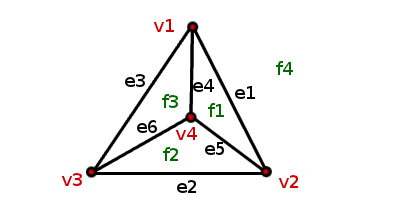
\includegraphics[scale=0.4]{mesh-r.png}
\\
\begin{table}[!h]
\begin{tabular}{|c||c|}
\hline
\textcolor{green}{f1} & \textcolor{red}{v1 v4 v2} \\ \hline
\textcolor{green}{f2} & \textcolor{red}{v2 v3 v4} \\ \hline
\textcolor{green}{f3} & \textcolor{red}{v3 v1 v4} \\ \hline
\textcolor{green}{f4} & \textcolor{red}{v1 v2 v3} \\ \hline
\end{tabular}
\end{table}
\\
\underline{\emph{winged-edge}}\\
\\
The representation consists of edge list, face list and vertex list.\\
Each face is given by two verticies and contains two references to faces around the edge.
The faces are explicitly represented by the set of edges. In the vertex list, each vertex contains
set of edges drawn from the vertex. This representation is redundant rather than the $F-V$ representation.
 This implementation fasten apparently fastens the query operations.\\
 
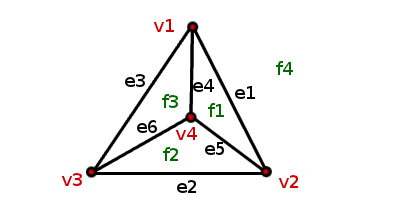
\includegraphics[scale=0.4]{mesh-r.png}
\\

\begin{tabular}{ c c c}
Vertex list & Edge list & Face list
\\
\begin{minipage}{0.3\columnwidth}
\raisebox{1.5cm}{
\begin{tabular}{|c||c|c|}
\hline
\textcolor{red}{v1} & e3 e4 e1\\ \hline
\textcolor{red}{v2} & e1 e2 e5\\ \hline
\textcolor{red}{v3} & e3 e2 e6\\ \hline
\textcolor{red}{v4} & e6 e4 e5\\ \hline
\end{tabular}}
\end{minipage}
&
\begin{minipage}{0.3\columnwidth}
\begin{tabular}{|c||c|c|}
e1 & \textcolor{red}{v1 v2} & \textcolor{green}{f1 f4} \\ \hline
e2 & \textcolor{red}{v3 v2} & \textcolor{green}{f2 f4} \\ \hline
e3 & \textcolor{red}{v1 v3} & \textcolor{green}{f3 f4} \\ \hline
e4 & \textcolor{red}{v1 v4} & \textcolor{green}{f1 f3} \\ \hline
e5 & \textcolor{red}{v2 v4} & \textcolor{green}{f1 f2} \\ \hline
e6 & \textcolor{red}{v3 v4} & \textcolor{green}{f2 f2} \\ \hline
\end{tabular}
\end{minipage}
&
\begin{minipage}{0.3\columnwidth}
\raisebox{1.6cm}{
\begin{tabular}{|c||c|}
\hline
\textcolor{green}{f1} & e1 e4 e5 \\ \hline
\textcolor{green}{f2} & e2 e5 e6 \\ \hline
\textcolor{green}{f3} & e3 e6 e4 \\ \hline
\textcolor{green}{f4} & e1 e2 e3 \\ \hline
\end{tabular}}
\end{minipage}

\end{tabular}


\newpage
\textbf{Operations}\\

\begin{tabular}{| c | c | c |}
\hline
\begin{minipage}[c][3.0cm]{0.2\hsize} makeVFS \end{minipage} & 
\raisebox{-1.0cm}{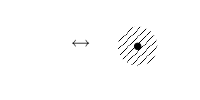
\includegraphics[scale=0.5]{makeVFS.png}} &
 killVFS\\ \hline
 
\begin{minipage}[c][3.0cm]{0.2\hsize} makeEV \end{minipage} & 
\raisebox{-1.0cm}{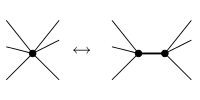
\includegraphics[scale=0.5]{makeEV.png}} & 
killEV\\ \hline

\begin{minipage}[c][3.0cm]{0.2\hsize} makeEF \end{minipage} & 
\raisebox{-1.0cm}{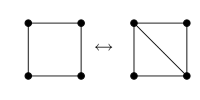
\includegraphics[scale=0.5]{makeEF.png}} & 
killEF\\ \hline

\begin{minipage}[c][3.0cm]{0.2\hsize} makeEkillR \end{minipage} & 
\raisebox{-1.0cm}{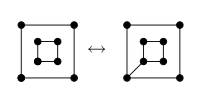
\includegraphics[scale=0.5]{makeEkillR.png}} & 
killRmakeE\\ \hline

\begin{minipage}[c][3.0cm]{0.2\hsize} makeFkillRH \end{minipage} &
\raisebox{-1.0cm}{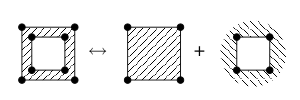
\includegraphics[scale=0.5]{makeFkillRH.png}} & 
killFmakeRH\\ \hline
\end{tabular}


%\begin{tabular}{ | c | c | c | }
%\multicolumn{1}{r}{}
% &  \multicolumn{1}{c}{\emph{vertex - face}}
% & \multicolumn{1}{c}{\emph{winged edge}} \\\hline
%\emph{makeVFS} & O(1) & O(1) \\ \hline
%\emph{makeEV} & O(F) & O(E) \\ \hline
%\emph{makeEF} & O(1) & O(1) \\ \hline
%\emph{makeEkillR} & O(F) & O(1) \\ \hline
%\emph{makeFkillRH} & O(1) & O(1) \\ \hline \hline
%\emph{splitE} & - & - \\ \hline
%\emph{joinE} & - & - \\ \hline
%\emph{splitF} & - & - \\ \hline
%\emph{joinF} & - & - \\ \hline
%\end{tabular}
%
%\\
\newpage
\underline{\emph{Truncate}}\\
\\
\emph{e.g.: Assuming $K_{4}$ graph}
\\
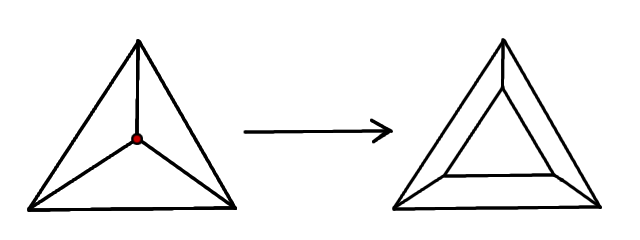
\includegraphics[scale=0.30]{truncate.png}
\\ \\
let the red vertex $v_{A}$ to be truncated\\
\\
\begin{tabular}{ l l }
\emph{vertex-face} & \emph{winged-edge}\\
\\
\raisebox{3.3cm}{\begin{minipage}{0.48\columnwidth}\fontsize{10pt}{10pt}
\textsl{Na začiatku musíme prejsť celý list facov a vybrať vrcholy, ktoré sa vyskytujú
 dvakrát spoločne s vrcholom $v_{A}$. Tak dostaneme list susedov. Ku každému prvku z listu $v_{i}$
 vytvoríme prvok $v_{i}^{*}$ ktorý pridáme do každého facu obsahujúci $v_{i}$. Nakoniec odstránime vrchol $v_{A}$ z listu a pridáme nový face obsahujúci všetky prvky $v_{i}^{*}$. Hľadanie suseda pre jeden vrchol môže
  mať zložitosť až $\mathcal{O}(F)$, takže celková zložitosť nám vystúpi až na $\mathcal{O}(V \times F)$.}
\end{minipage}} &

\begin{minipage}{0.48\columnwidth}
\textsl{V tejto reprezentácií dokážeme určiť všetky hrany vedúce z vrcholu v
konštantnom čase.(V ideálnom prípade. Zložitosť je priamo závislá na reprezentácií
zoznamu hrán a vrcholov.) Odtiaľ v závislosti na počte hrán dokážeme určiť všetky susedné
vrcholy. Podobne ako v prvom prípade, pre každý susedný vrchol $v_{i}$ vytvoríme nový vrchol $v_{i}^{*}$ z ktorého vytvoríme nový face. Predtým, ako vytvoríme nový face, potrebujeme zaznamenať vytvorené hrany. 
Pre operáciu $truncate$ si môžeme definovať homomorfizmus $f:v_{i} \rightarrow v_{i}^{*}$, kde platí $e(v_{i},v_{j})=e(v_{i}^{*},v_{j}^{*})$. Odtiaľ v čase $\mathcal{O}(E^{2})$ vytvoríme zoznam hrán, ktoré
tvoria nový face. Face pridáme do zoznamu a do zoznamu hrán pridáme nové hrany, ku ktorým zapíšeme referenciu na nový face a na face, ktorý patrí hrane $e(v_{i},v_{j}$ z ktorej bola hrana $e(v_{i}^{*},v_{j}^{*})$
vytvorená. Nakoniec v každej hrane $e(v_{i},v_{A})$ zmeníme vrchol $v_{A}$ na $v_{i}^{*}$. Celková zložitosť bude $\mathcal{O}(E^{2})$ za predpokladu, že všetky zoznamy máme v štandarnom poli.}

\end{minipage}

\end{tabular}


\newpage
\underline{\emph{bevel}}\\
\\
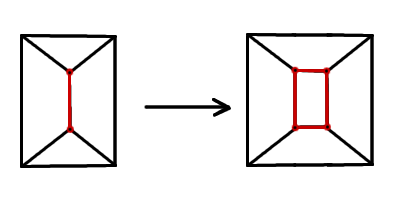
\includegraphics[scale=0.40]{bevel.png}\\
\\
let red vertecies $v_{A}$ and $v_{B}$ to be beveled\\
\\
\begin{tabular}{ l l }
\emph{vertex-face} & \emph{winged-edge}\\
\\
\raisebox{1.5cm}{
\begin{minipage}{0.48\columnwidth}\fontsize{10pt}{10pt}
\textsl{operácia bude asymptoticky časovo rovnako náročná}
\end{minipage}} &

\begin{minipage}{0.48\columnwidth}
\textsl{operácia bude asymptoticky časovo rovnako náročná ako truncate. Rozdiel bude len v tom, že
že na začiatku do zoznamu nových vrcholov pridáme všetkých susedov $v_{A}$ a $v_{A}$ a odtiaľ postupujeme
rovnako ako v operácií truncate. V prípade, že na vstupe máme len ukázateľ na hranu, vrcholy
$v_{A}$ a $v_{B}$ dokážeme nájsť v konštantnom čase.}

\end{minipage}

\end{tabular}

\newpage
\textbf{Advanced mesh operations}
\\

V tejto sekcii popisujem náväznosť základných \emph{Eulerových operácií} na komplikovanejšie operácie, ktoré dokážu
meniť tvar \emph{meshu} oveľa efektívnejšie.\\

%\emph{\underline{makeEV}, \underline{makeEF}, (\underline{makeVFS})}\\

%Na tieto operácie nadväzujú pochopiteľne úpravy z kategórie \textsf{add}.\\



\begin{table}[!h]
\centering
\begin{tabular}{|c|c|c|c|c|c|c|}
\hline
 & \textbf{makeVFS} & \textbf{makeEV} & \textbf{makeEF} 
 & \textbf{killVFS} & \textbf{killEV} & \textbf{killEF}\\ 
\hline
\emph{extrude} 
& ? 
&  \multicolumn{1}{>{\columncolor{softred}}p{0.15\columnwidth}|}{\centering required} 
&  \multicolumn{1}{>{\columncolor{softred}}p{0.15\columnwidth}|}{\centering required} 
& - & - & - \\

\hline
\emph{subdivide} 
& ? 
&  \multicolumn{1}{>{\columncolor{softred}}p{0.15\columnwidth}|}{\centering required} 
&  \multicolumn{1}{>{\columncolor{softred}}p{0.15\columnwidth}|}{\centering required} 
& - & - & - \\

\hline
\emph{bevel} 
& ? 
&  \multicolumn{1}{>{\columncolor{softred}}p{0.15\columnwidth}|}{\centering required} 
&  \multicolumn{1}{>{\columncolor{softred}}p{0.15\columnwidth}|}{\centering required} 
& - & - & - \\

\hline
\emph{truncate} 
& ? 
&  \multicolumn{1}{>{\columncolor{softred}}p{0.15\columnwidth}|}{\centering required} 
&  \multicolumn{1}{>{\columncolor{softred}}p{0.15\columnwidth}|}{\centering required} 
& - & - & - \\

\hline
\hline
\emph{delete faces} 
& - & - & -
& ? 
&  \multicolumn{1}{>{\columncolor{softred}}p{0.15\columnwidth}|}{\centering required} 
&  \multicolumn{1}{>{\columncolor{softred}}p{0.15\columnwidth}|}{\centering required}  \\

\hline
\emph{delete edges} 
& - & - & -
& ? 
&  \multicolumn{1}{>{\columncolor{softred}}p{0.15\columnwidth}|}{\centering required} 
&  \multicolumn{1}{>{\columncolor{softred}}p{0.15\columnwidth}|}{\centering required}  \\

\hline
\emph{delete verticies} 
& - & - & -
&  \multicolumn{1}{>{\columncolor{softred}}p{0.15\columnwidth}|}{\centering required}
&  \multicolumn{1}{>{\columncolor{softred}}p{0.15\columnwidth}|}{\centering required} 
&  \multicolumn{1}{>{\columncolor{softred}}p{0.15\columnwidth}|}{\centering required}  \\


\hline
\emph{merge} 
& - & - & -
& ? 
&  \multicolumn{1}{>{\columncolor{softred}}p{0.15\columnwidth}|}{\centering required} 
&  \multicolumn{1}{>{\columncolor{softred}}p{0.15\columnwidth}|}{\centering required}  \\

\hline
\hline

\emph{scale} 
& - & - & -
& - & - & -  \\
\hline

\emph{translate} 
& - & - & -
& - & - & -  \\
\hline

\emph{rotate} 
& - & - & -
& - & - & -  \\
\hline

\rowcolor{blue}
\end{tabular}
\end{table}

\newpage

\begin{figure}[!h]
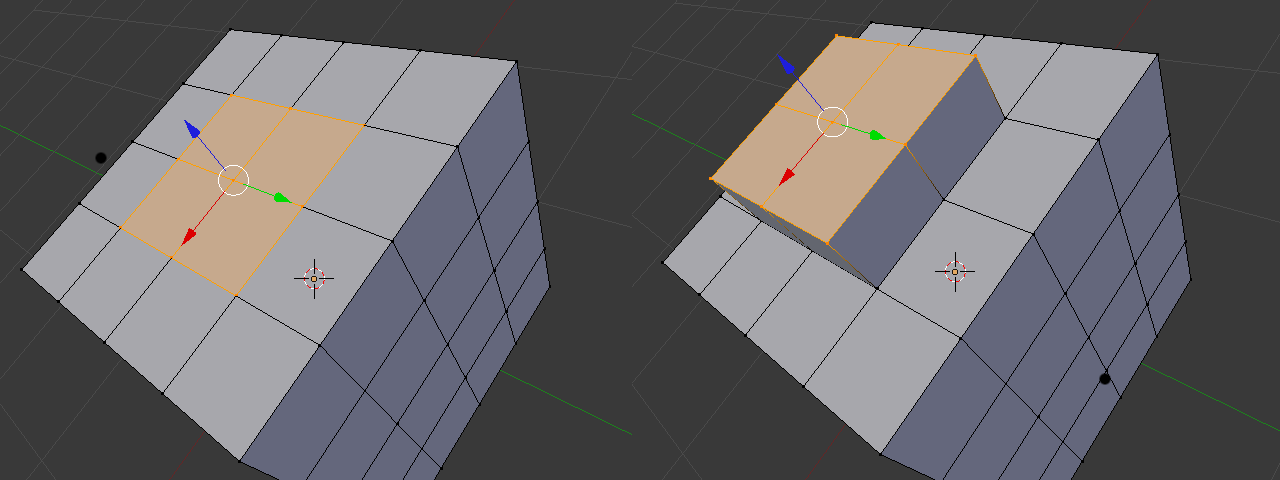
\includegraphics[scale=0.25]{extrude.png}
\caption{extrude}
\end{figure}

\begin{figure}[!h]
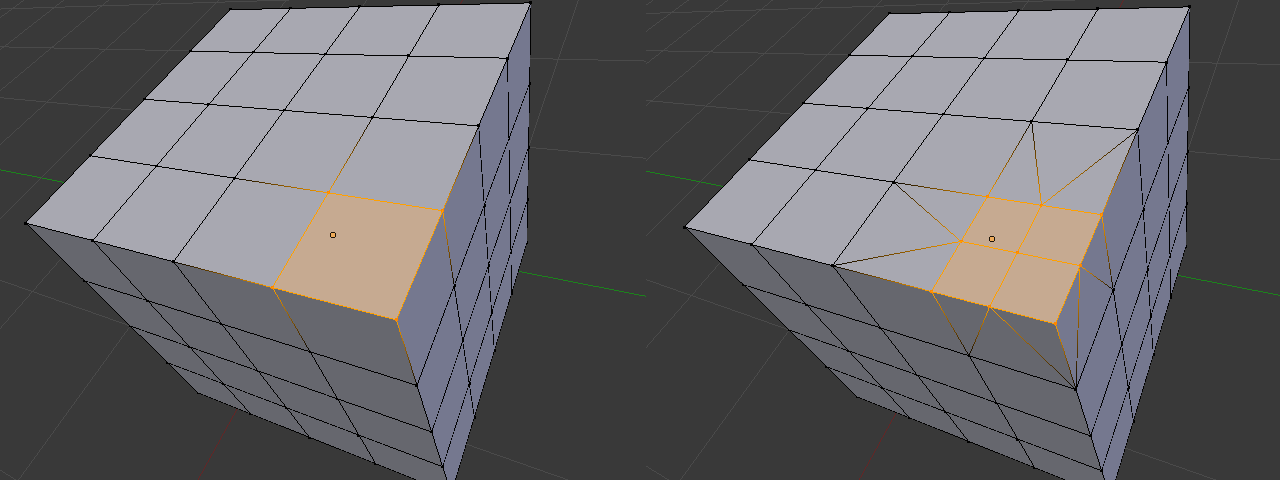
\includegraphics[scale=0.25]{subdivide.png}
\caption{subdivide}
\end{figure}

\begin{figure}[!h]
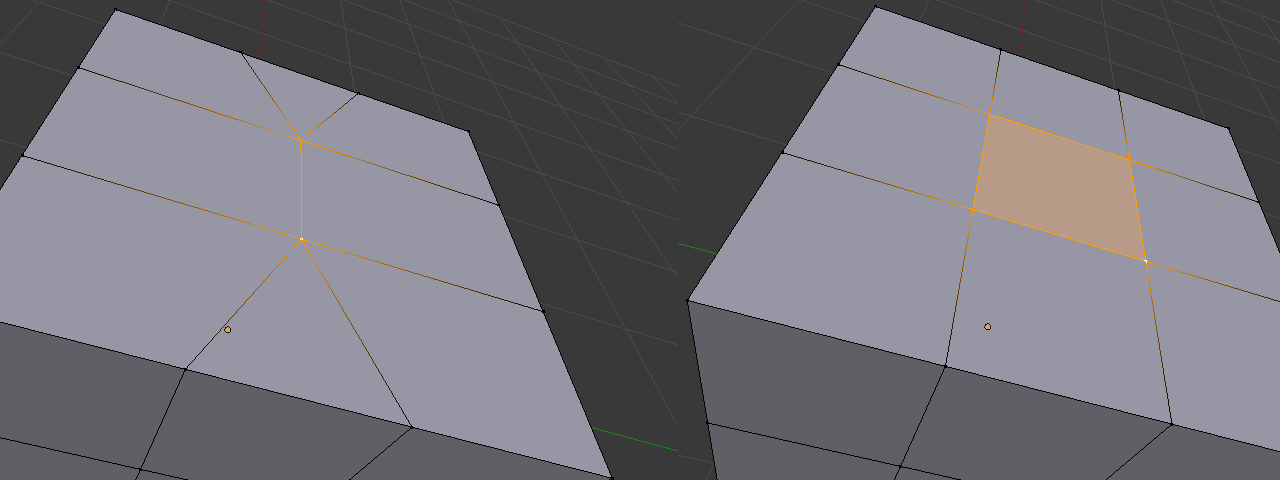
\includegraphics[scale=0.25]{bevel1.png}
\caption{bevel}
\end{figure}

\newpage

\begin{figure}[!h]
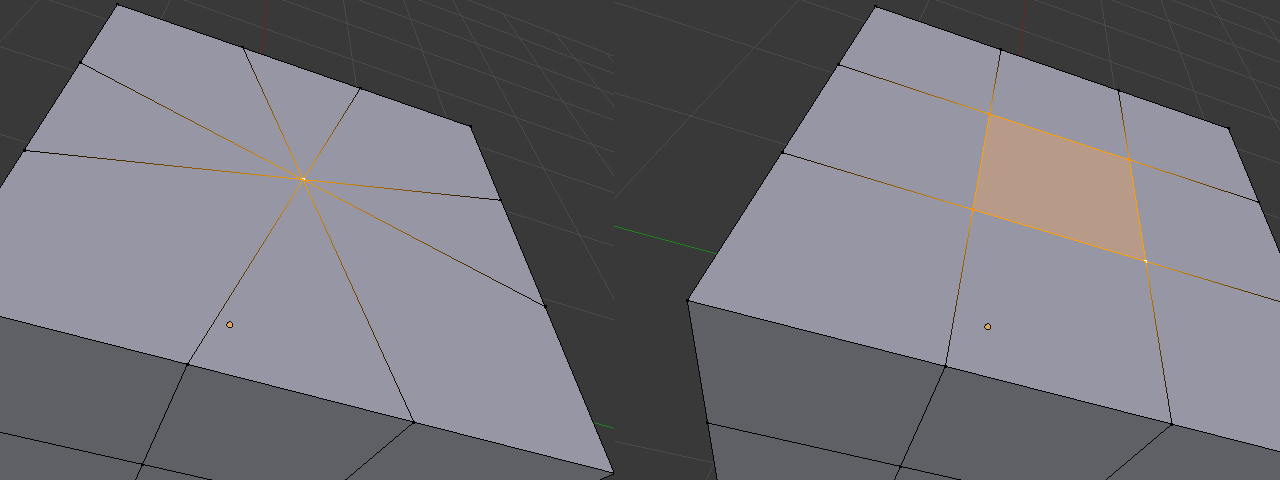
\includegraphics[scale=0.25]{truncate1.png}
\caption{truncate}
\end{figure}

\begin{figure}[!h]
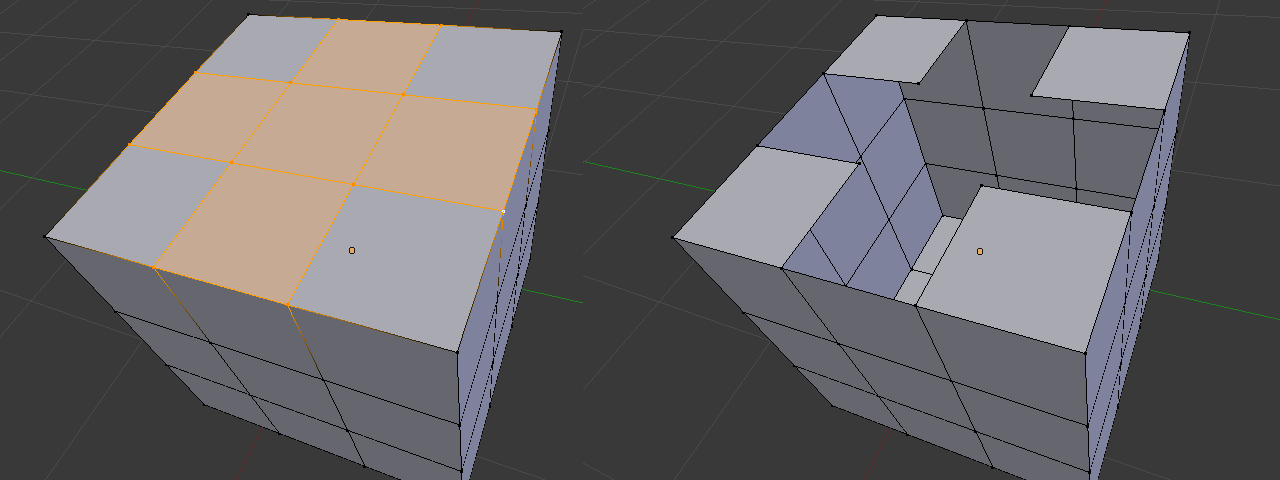
\includegraphics[scale=0.25]{deleteF.png}
\caption{delete faces}
\end{figure}

\newpage

\textbf{Concept}
\\

\begin{tabular}{p{0.2\textwidth} r}

\multicolumn{1}{>{\columncolor{white}} p{0.5\columnwidth}}{\textsf{\textcolor{darkgreen}{M}}} & \emph{a type representing the mesh}\\
\textsf{\textcolor{red}{m, v, e, f}} & \emph{instances (mesh, vertex, edge, face)}
%DO PEKLA AJ S ČIRNOU BUNKOU!!
\end{tabular}


\begin{itemize}

\item \emph{Mesh (top level)}

\begin{table}[0.8\textwidth]
\begin{tabular}{| p{0.55\columnwidth} | p{0.5\columnwidth} |}
\hline
\textsf{\textcolor{darkblue}{mesh\_traits\textless}\textcolor{darkgreen}{M}\textcolor{darkblue}{\textgreater ::vertex\_descriptor}}  &
\emph{Type for vertex object}\\ \hline

\textsf{\textcolor{darkblue}{mesh\_traits\textless}\textcolor{darkgreen}{M}\textcolor{darkblue}{\textgreater ::face\_descriptor}} & \emph{Type for face object}\\ \hline
\textsf{\textcolor{brown}{static} \textcolor{darkred}{bool}} \textsf{\textcolor{darkblue}{is\_trimesh(\textcolor{red}{m})}} &  \emph{checks whether the datatype is restricted to be a triangle mesh}\\ \hline
\end{tabular}
\end{table}

\item \emph{Face-Vertex (refines Mesh)}
\begin{table}[0.8\textwidth]
\begin{tabular}{|p{0.55\columnwidth} | p{0.5\columnwidth} |} 

\hline
\textsf{\textcolor{darkblue}{mesh\_traits\textless}\textcolor{darkgreen}{M}\textcolor{darkblue}{\textgreater ::vertex\_iterator}} & \emph{Iterate through all vertices}\\ \hline

\textsf{\textcolor{darkblue}{mesh\_traits\textless}\textcolor{darkgreen}{M}\textcolor{darkblue}{\textgreater ::vertices\_size\_type}} & \emph{Type for number of vertices}\\ \hline

\textsf{\textcolor{darkred}{vertices\_size\_type}} \textsf{\textcolor{darkblue}{vertices\_size(\textcolor{red}{m})}} & \emph{get number of vertices}\\ \hline

\textsf{\textcolor{darkblue}{mesh\_traits\textless\textcolor{darkgreen}{M}\textgreater ::face\_iterator}} & \emph{Iterate through all faces}\\ \hline

\textsf{\textcolor{darkblue}{mesh\_traits\textless\textcolor{darkgreen}{M}\textgreater ::faces\_size\_type}} & \emph{Type for number of faces}\\ \hline

\textsf{\textcolor{darkred}{faces\_size\_type}} \textsf{\textcolor{darkblue}{faces\_size(\textcolor{red}{m})}} & \emph{get number of faces} \\ \hline

\textsf{\textcolor{darkblue}{mesh\_traits\textless\textcolor{darkgreen}{M}\textgreater ::fv\_iterator}} & \emph{iterate through vertices contained in the face (face-vertex iterator)} \\ \hline

\textsf{\textcolor{purple}{std::pair\textless\textcolor{darkred}{fv\_iterator,fv\_iterator}\textgreater}\, \hspace*{2.5px} \textcolor{darkblue}{get\_vertices\_from\_face(\textcolor{red}{m}, \textcolor{red}{f})}} &  \emph{get all vertices contained in the face} \textsf{f} \\ \hline

\textsf{\textcolor{darkred}{bool} \textcolor{darkblue}{add\_vertex( ??? )}} & \emph{TODO data structure - \textcolor{red}{prekonzultovať}} \\ \hline
\textsf{\textcolor{darkred}{bool} \textcolor{darkblue}{add\_face( ??? )}} & \emph{TODO data structure - \textcolor{red}{prekonzultovať}} \\ \hline
\textsf{\textcolor{darkred}{bool} \textcolor{darkblue}{remove\_face( ??? )}} & \emph{TODO data structure - \textcolor{red}{prekonzultovať}} \\ \hline


\end{tabular}
\end{table}
\newpage
\item \emph{Winged-edge (refines Face-Vertex)}
\begin{table}[!h]
\begin{tabular}{| p{0.55\columnwidth} | p{0.5\columnwidth} |}
\hline
\textsf{\textcolor{darkblue}{mesh\_traits\textless\textcolor{darkgreen}{M}\textgreater ::edge\_descriptor}} & \emph{Type for edge object}\\ \hline

\textsf{\textcolor{darkblue}{mesh\_traits\textless\textcolor{darkgreen}{M}\textgreater ::edge\_iterator}} & \emph{Iterate through all edges}\\ \hline

\textsf{\textcolor{darkblue}{mesh\_traits\textless\textcolor{darkgreen}{M}\textgreater ::edges\_size\_type}} & \emph{Type for number of edges}\\ \hline

\textsf{\textcolor{darkred}{edges\_size\_type}} \textsf{\textcolor{darkblue}{edges\_size(\textcolor{red}{m})}} & \emph{get number of edges}\\ \hline

\textsf{\textcolor{purple}{std::pair\textless\textcolor{darkred}{face\_descriptor,face\_descriptor}\textgreater}, \hspace*{2.5px} \textcolor{darkblue}{get\_faces\_from\_edge(\textcolor{red}{m}, \textcolor{red}{e})}} &  \emph{get (2) faces around edge} \textsf{e} \\ \hline

\textsf{\textcolor{purple}{std::pair\textless\textcolor{darkred}{vertex\_descriptor,vertex\_descriptor}\textgreater}\, \hspace*{2.5px} \textcolor{darkblue}{get\_vertices\_from\_edge(\textcolor{red}{m}, \textcolor{red}{e})}} &  \emph{get (2) vertices of edge} \textsf{e} \\ \hline

\textsf{\textcolor{darkblue}{mesh\_traits\textless\textcolor{darkgreen}{M}\textgreater ::vv\_iterator}} & \emph{iterate through vertices adjacent to the vertex (vertex-vertex iterator)} \\ \hline

\textsf{\textcolor{purple}{std::pair\textless\textcolor{darkred}{vv\_iterator,vv\_iterator}\textgreater}\, \hspace*{2.5px} \textcolor{darkblue}{get\_adjacent\_vertices(\textcolor{red}{m}, \textcolor{red}{v})}} &  \emph{get all vertices adjacent to vertex} \textsf{v} \\ \hline

\textsf{\textcolor{darkblue}{mesh\_traits\textless\textcolor{darkgreen}{M}\textgreater ::fe\_iterator}} & \emph{iterate through edges surrounding the face (face-edge iterator)} \\ \hline

\textsf{\textcolor{purple}{std::pair\textless\textcolor{darkred}{fe\_iterator,fe\_iterator}\textgreater}\, \hspace*{2.5px} \textcolor{darkblue}{get\_surrounding\_edges(\textcolor{red}{m}, \textcolor{red}{f})}} &  \emph{get all edges around the face} \textsf{f} \\ \hline

\textsf{\textcolor{darkred}{bool} \textcolor{darkblue}{add\_edge( ??? )}} & \emph{TODO data structure - \textcolor{red}{prekonzultovať}} \\ \hline

\textsf{\textcolor{darkred}{bool} \textcolor{darkblue}{remove\_edge( ??? )}} & \emph{TODO data structure - \textcolor{red}{prekonzultovať}} \\ \hline

\textsf{\textcolor{darkred}{bool} \textcolor{darkblue}{remove\_vertex( ??? )}} & \emph{TODO data structure - \textcolor{red}{prekonzultovať}} \\ \hline

\end{tabular}
\end{table}


\end{itemize}

\begin{figure}[!h]
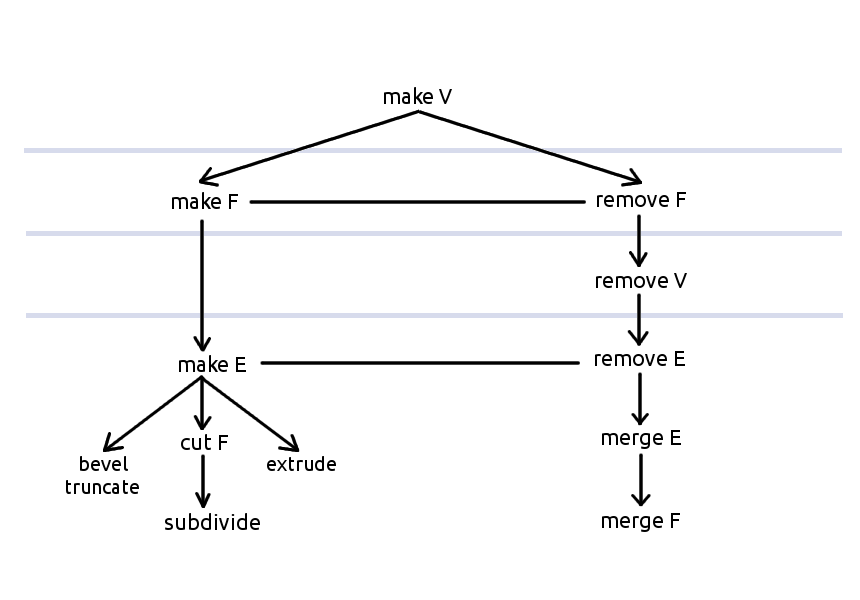
\includegraphics[scale=0.5]{hierarchy.png}
\caption{operation hierarchy}
\end{figure}
%
%\begin{table}[0.8\textwidth]
%	\begin{tabular}{| p{0.25\columnwidth} || p{0.8\columnwidth} |}
%	\hline \textsf{Mesh} & Basic mesh concept\\
%	\hline
%	\hline \textsf{Iterable\_Vertices} & \\
%	\hline \textsf{Iterable\_Edges} & \\
%	\hline \textsf{Iterable\_Faces} & \\
%	\hline 
%	\hline \textsf{Makeable\_Vertices} & \\
%	\hline \textsf{Makeable\_Edges} & \\
%	\hline \textsf{Makeable\_Faces} & \\
%	\hline
%	\hline \textsf{Removable\_Vertices} & \\
%	\hline \textsf{Removable\_Edges} & \\
%	\hline \textsf{Removable\_Faces} & \\
%	\hline
%	\hline \textsf{Cutable\_Faces} & \\
%	\hline \textsf{Extrudable\_Submesh} & \\
%	\hline
%	\hline \textsf{Mergeable\_Edges} & \\
%	\hline \textsf{Mergeable\_Faces} & \\
%	\hline
%	\end{tabular}
%\end{table}

\newpage

\textbf{Implementácia}
\\


\textsc{mesh\_traits\textless Mesh\textgreater}
\\

Trieda, ktorá je používaná v jednotlivých algoritmoch pre našu implementáciu mesh-e. Obsahuje základné typy a operácie nad meshom
v závislosti, čo algoritmus vyžaduje, resp. jeho koncept.
\\


\textsc{advanced\_mesh\_traits\textless Mesh\textgreater}
\\

Špeciálna varianta triedy, ktorá je popísaná vyššie. Okrem základných operácií, ktoré získa oddedením, je doplnená o operácie, ktoré
implementácia štandardne nepodporuje (e.g. dotaz na susedný vrchol v implementácií \emph{Face-Vertex}). Používa sa len v špeciálnych
prípadoch. Jej značnou nevýhodou je spomalenie algoritmov.
\\
\newpage

\textsc{Class winged\_edge\_mesh}
\\

Vlastná implementácia mesh\-e, podľa špecifikácie \emph{winged\_edge} s redundantnými normálami. Obsahuje subtriedy \emph{vertex}, \emph{edge}, \emph{face}, \emph{normal} a \emph{vv\_iterator}. Implementácia používa containery \emph{std::vector\textless T\textgreater}
a ich príslušné iterátory.
\\

\textsc{Class OpenMeshExtended}
\\
\\
Je to knihovná trieda, ktorá je dodatočne šablónovaná následovne.\\
\\
\textsf{
struct MyTraits : public OpenMesh::DefaultTraits\\
\{\\
 VertexAttributes(OpenMesh::Attributes::Status);\\
 FaceAttributes(OpenMesh::Attributes::Status);\\
 EdgeAttributes(OpenMesh::Attributes::Status);\\
\};\\
\\
OpenMesh::PolyMesh\_ArrayKernelT\textless MyTraits\textgreater
}\\
\\
Na začiatok podľa špecifikácie OpenMesh je nutné priradiť mesh-u atribúty, ktoré nám umožňujú pridávať a odoberať prvky meshu.
Trieda na rozdiel od \emph{winged\_edge\_mesh} si nedrží informáciu o stave normály, ale pri každom dotaze na normálu steny smer vypočíta
z vektorového súčinu vrcholov, ktorý stenu tvoria.\\
\\
Implementácia používa špeciálne vlastné iterátory, pre iteráciu po celej štruktúre a pre dotazy na prvky v okolí(napr. \emph{FaceVertexIterator} pre dotaz na vrcholy, ktoré patria príslušnej stene).
\\
\\

\textbf{Algoritmy}
\\

\textsc{Compute componets\textless Mesh, MeshTraits\textgreater}\\
\\
Je to jednoduchý algoritmus, šablónovaný mesh-om a jeho trait-ami, ktorý spočíta komponenty pomocou upraveného algoritmu BFS.
Samostatný izolovaný vrchol považuje ako jednu komponentu.
\\

\textsc{Flip normals\textless Mesh, MeshTraits\textgreater}\\
\\
Algoritmus, ktorý prechádza všetky steny a otáča im normály. V tomto prípade musí implementácia OpenMeshExtended používať
advanced traits, nakoľko defaultne nepodporuje otáčanie normály pre jednu stenu. 
V rozšírených trait-och je to implementované pomocou výmeny hrán.

\end{document}
